\chapter{Polarisation, réflexion, réfraction}

\section{Polarisation} 

La \textit{polarisation d'une onde électromagnétique} est le lieu décrit au cours du temps à un endroit donné de l'espace par l'extrémité du vecteur champ
électrique associé à cette onde. Ce concept est inhérent aux ondes \textbf{transverses}. 
Dans le cadre de ce cours, nous allons nous intéresser aux ondes EM transverses planes afin d'analyser la polarisation de l'onde «facilement» étant donné que le vecteur champ électrique sera toujours
contenu dans un plan et que les plans successifs sont tous parallèles. 

\subsection{Expression générale du champ électrique d'une onde EM transverse plane}
\begin{marginfigure}
	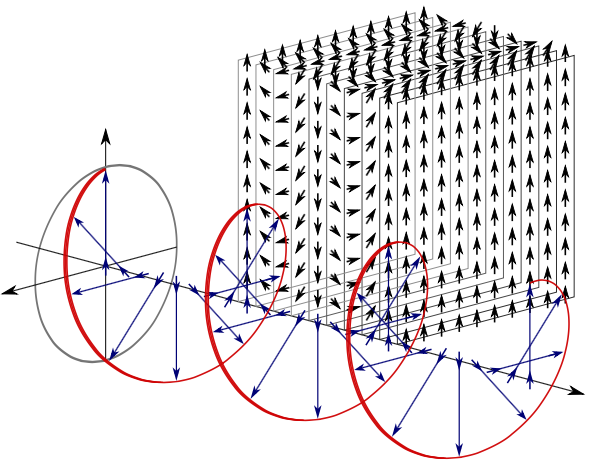
\includegraphics[width = \linewidth]{polarisationL.png}
	\caption{Illustration de la polarisation circulaire d'une onde plane Nous pouvons en effet observer que le lieu décrit par la pointe du vecteur E est un cercle.}
\end{marginfigure}
Avec la définition que nous venons de donner, nous pouvons simplement écrire (pour des plans d'équation : $ z = ||\vec{r}||$) 

\[\vec{E}(\vec{r},t) = A_{x} \sin(\vec{k}\cdot \vec{r} - \omega t) \hat{x} + A_{y} \sin(\vec{k}\cdot \vec{r} - \omega t + \phi) \hat{y}\] 

où $\vec{r} = (x,y,z)$ représente les coordonnées cartésiennes du point considéré, $\phi$ est le \textbf{déphasage} angulaire entre 
la composante en Y
et la composante en X.

Si $A_{x},A_{y}, \phi$ 
sont quelconques, la polarisation est dite
 \textit{\textbf{elliptique}}
et cela se vérifie facilement.\\
Dans le cas particulier où $\phi = n \pi$, l'effet du déphasage n'est plus perceptible réellement car nous aurions, en fonction 
de $n$ pair ou impair, un second terme valant en norme $\pm A_{y} \sin(\vec{k}\cdot \vec{r} - \omega t)$.

Dès lors, nous pourrions regrouper les deux sinus en un seul dans une direction de pente 1 en X et Y car nous aurions une combinaison 
des vecteurs unitaires $\hat{x}$ et $\hat{y}$. Dans ce cas-là, la polarisation devient \textit{\textbf{linéaire}}.

Dans le cas particulier où $\phi = \frac{(2n+1) \pi }{2}$ \textbf{et} la valeur absolue des amplitudes $A_{x}, A_{y}$ est identique, 
nous avons affaire, par le même genre de raisonnement, à une polarisation \textit{\textbf{circulaire}} (voir image\footnote{Source: \url{https://fr.wikipedia.org/wiki/Onde_plane}}). 
En effet, le second terme devient ici un cosinus de même pulsation angulaire et son amplitude vaut $\pm A_{x}$. 


\section{Réflexion et réfraction} 

\subsection{Mise en route: réflexion et transmission d'une onde mécanique le long d'une corde} 

\begin{figure*}
	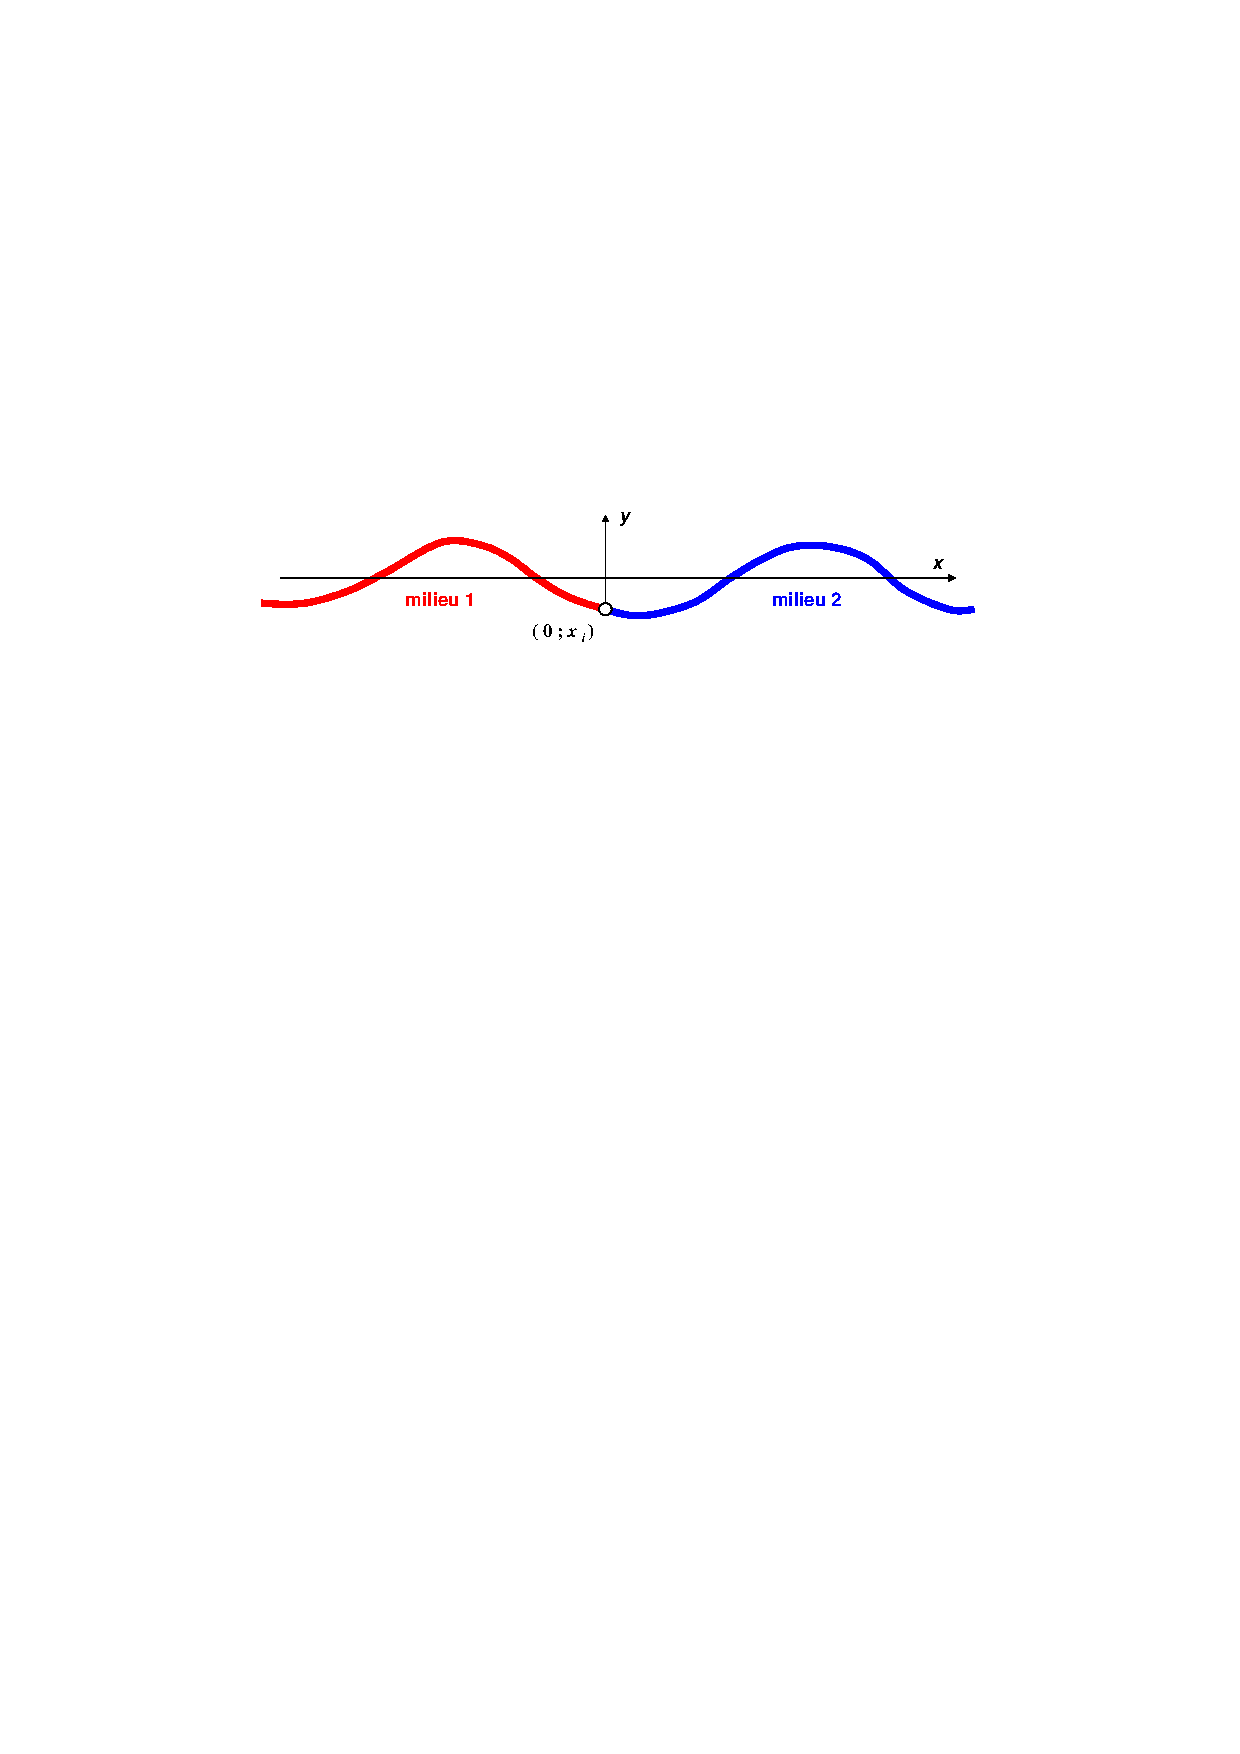
\includegraphics[width=\linewidth]{CM4_condlimite}
	\caption{L'interface de la corde tendue.}
\end{figure*}
Avant de développer le cas des ondes EM, étudions la transmission (et la réflexion qui en résulte forcément) d'une onde \textit{mécanique} transversale d'un milieu défini par les paramètres $({F}_1,{\mu_1})$ à un autre défini par $({F}_2,{\mu_2})$ (pour rappel, $F$ est la tension dans la corde et $\mu_i$, dans le contexte de la corde, représente sa masse par unité de longueur; la vitesse de phase s'exprime par $v_i = \sqrt{\frac{F_i}{\mu_i}}$, et le nombre d'onde $k_i = \omega/v_i$, $i = 1, 2$). Cette vitesse change d'un milieu à un autre.\\
L'onde \textit{incidente} (c.-à-d. l'onde avant qu'elle ne rencontre l'interface) peut s'écrire sous forme scalaire

\[ \xi_{1i}(x,t) = I \sin(k_{1}x - \omega t) \]

L'onde réfléchie et l'onde transmise auront pour équations respectives\footnote{-$k_{1}$ dénote bien que l'onde réfléchie se déplace dans la direction opposée par rapport à l'onde incidente.} : 
\[ \xi_{1r}(x,t) = R \sin(-k_{1}x - \omega t) \]
\[ \xi_{2t}(x,t) = T \sin(k_{2}x - \omega t) \]

\textit{Les conditions aux interfaces impliquent ici la continuité du déplacement vertical de la corde $\xi$ et la continuité de la force 
verticale $F_y$}. L'application de ces conditions de continuité en $x=0$ résulte en un système de 2 équations à 2 inconnues $(R,T)$\footnote{La 2e relation s'obtient via la formule $F_y(0,t) = -F\:\frac{\partial \xi}{\partial x}(0,t)$ développée à la section \ref{corde_vibrante}, pour laquelle $y$ et $\xi$ sont identiques et correspondent au déplacement vertical de la corde.} :
\begin{align*}
    \xi_{1i}(0,t) + \xi_{1r}(0,t) = \xi_{2t}(0,t) &\Leftrightarrow I + R = T\\
    F_{y,1i}(0,t) + F_{y,1r}(0,t) = F_{y,2t}(0,t) &\Leftrightarrow k_{1}I - k_{1}R = k_{2}T
\end{align*}

Nous obtenons trivialement pour chaque inconnue les relations suivantes : 

\[R = \frac{k_{1} - k_{2}}{k_{1} + k_{2}}I\]
\[T = \frac{2 k_{1}}{k_{1} + k_{2}}I\]

On observe que tant l'onde transmise que l'onde réfléchie dépendent des caractéristiques des deux tronçons de corde !


\subsection{Réflexion et réfraction d'une onde EM} 

Nous pouvons transposer l'analyse ci-dessus aux ondes électromagnétiques, afin de décrire leur comportement à l'interface entre un milieu 1 ($\epsilon_{1}, \mu_{1}$) et un milieu 2 ($\epsilon_{2},\mu_{2}$), chaque milieu étant caractérisé par sa \textit{\textbf{perméabilité magnétique}} $\mu_i$
et sa \textbf{\textit{permittivité électrique}} $\epsilon_i$.

Pour rappel, la vitesse\footnote{Vitesse dite de \textit{phase}.} d'une onde électromagnétique vaut  

\[v = \frac{1}{\sqrt{\epsilon \mu}}\ = \frac{1}{\sqrt{\epsilon_{r} \mu_{r}}} \frac{1}{\sqrt{\epsilon_{0} \mu_{0}}} = \frac{1}{\sqrt{\epsilon_{r} \mu_{r}}} c,  \] 

et l'impédance caractéristique est définie par 

\[Z = \sqrt{\frac{\mu}{\epsilon}} = \sqrt{\frac{\mu_0\mu_r}{\epsilon_0\epsilon_r}} = Z_0 \sqrt{\frac{\mu_r}{\epsilon_r}}.  \]

On peut également définir l'indice de réfraction comme le rapport $n = c/v = \sqrt{\epsilon_{r}\mu_r}$.

Une onde, lorsqu'elle passe d'un milieu à un autre, conserve sa \textbf{fréquence}. La longueur d'onde (et donc le nombre d'onde) sont quant à eux tous affectés 
par le changement de milieu car ils dépendent directement de la vitesse de l'onde.


Afin de clarifier les choses, les différentes notations que nous allons utiliser sont reprises à la figure \ref{fig_CM4_conventions_k}.
\begin{marginfigure}
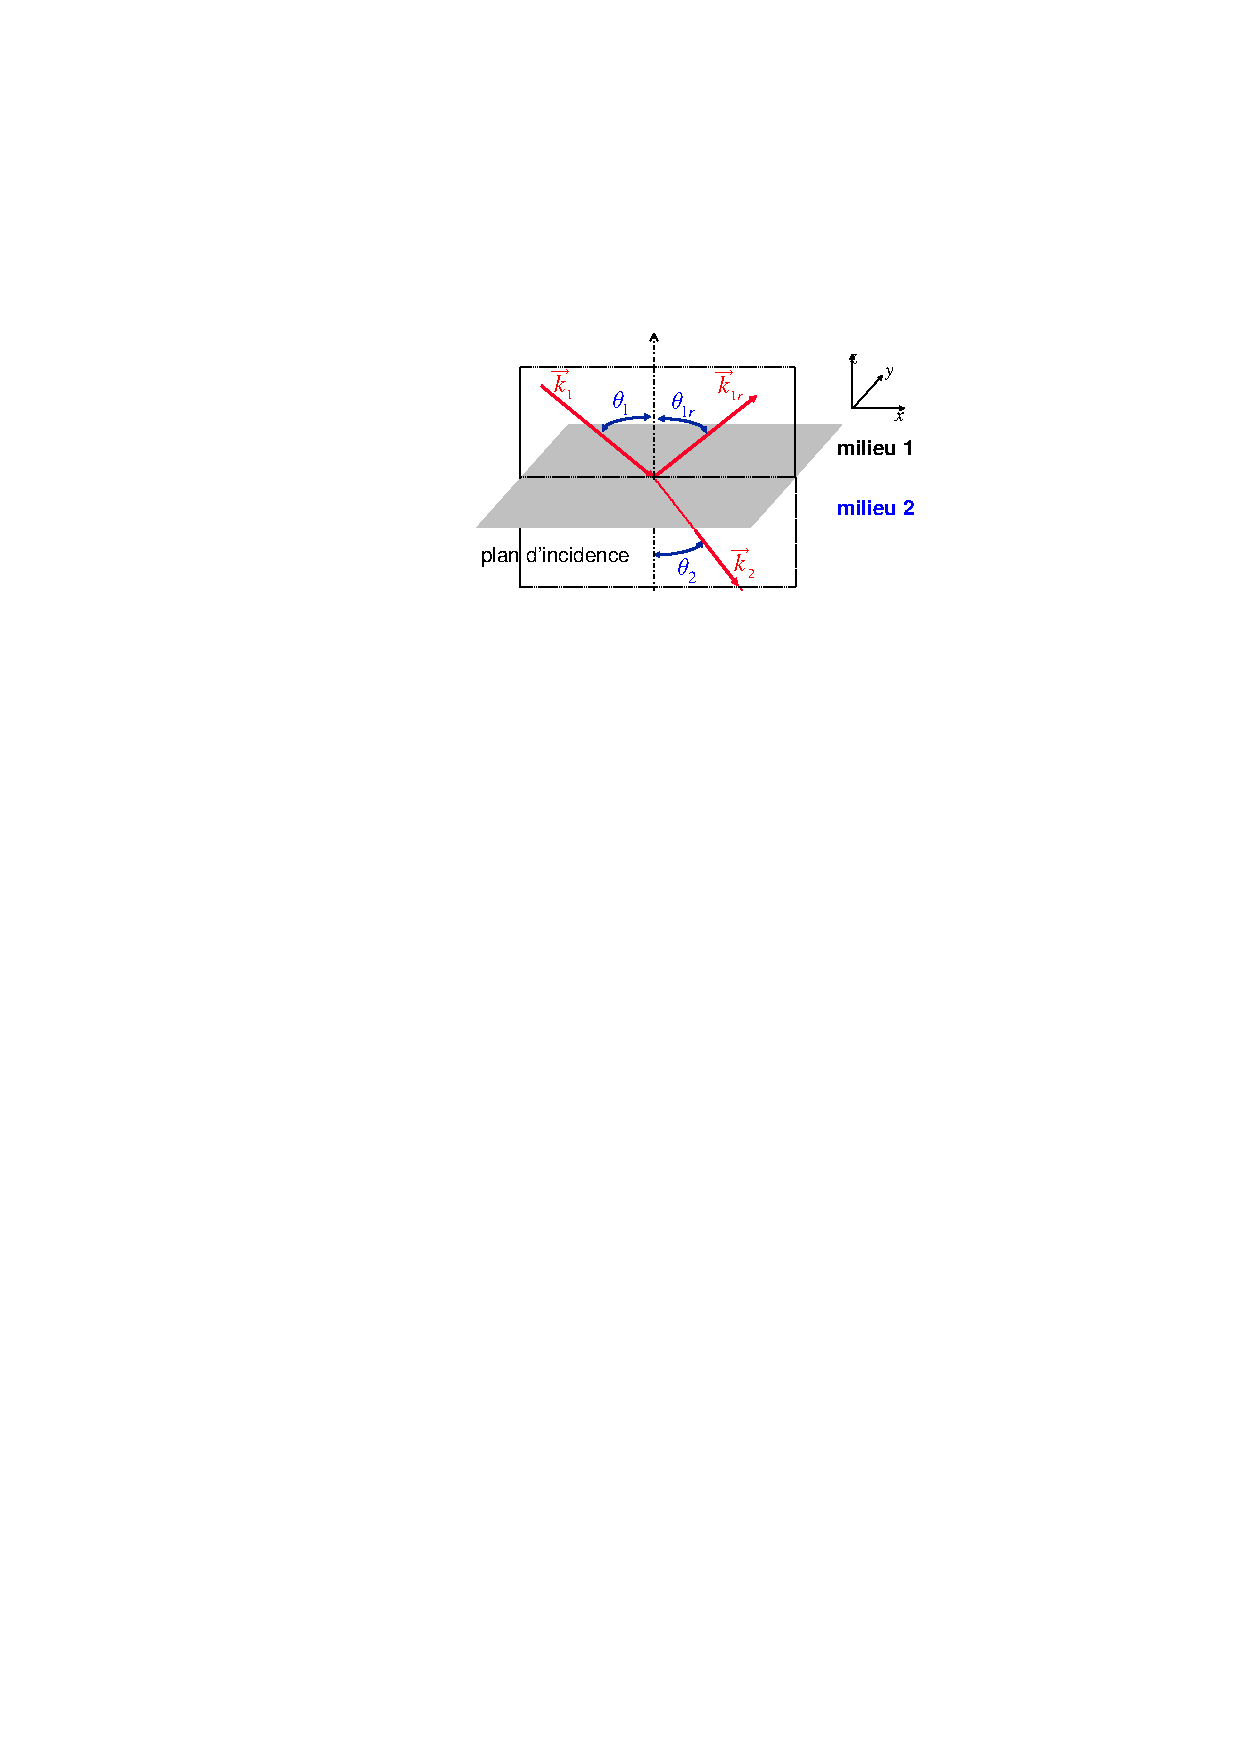
\includegraphics[width = \linewidth]{CM4_conventions_k}
\caption{Le plan d'incidence est le plan qui est formé de deux des 3 vecteurs d'ondes. (Ces 3 vecteurs d'onde sont coplanaires, le plan d'incidence sera donc la même si l'on prend le vecteur incident et réfléchi ou incident et transmis par exemple.)\\
Les caractéristiques de l'onde \textbf{incidente} seront notés avec un indice $1$ ou $1i$.\\
Les caractéristiques de l'onde \textbf{réfléchie} seront notés avec un indice $1r$ ou $r$. \\
Les caractéristiques de l'onde \textbf{transmise} seront notés avec un indice $2$ ou $2t$. \\
\textbf{Les angles sont toujours mesurés par rapport à la normale de l'interface!}}
\label{fig_CM4_conventions_k}
\end{marginfigure}

On peut tout d'abord montrer que l'angle d'\textit{incidence} vaut l'angle de \textit{réflexion}. 

\subsection{Loi de Snell}

Tout d'abord, nous avons les relations  $c = n_{1} v_{1} = n_{2} v_{2}$ et donc $\lambda_{1} n_{1}= \lambda_{2} n_{2}$.
De plus, les conditions aux interfaces imposent que la vitesse et donc le déplacement tangentiel à l'interface doit être le même.

Dès lors, (voir photo) les deux longueurs $L$ sont identiques. Par trigonométrie élémentaire, nous reportons les angles $\theta_{1}$ et $\theta_{2}$ 
dans les triangles rectangles et écrivons : $\mathcal{L} = \frac{\lambda_{1}}{\sin(\theta_{1})} = \frac{\lambda_{2}}{\sin(\theta_{2})}$

\begin{marginfigure}
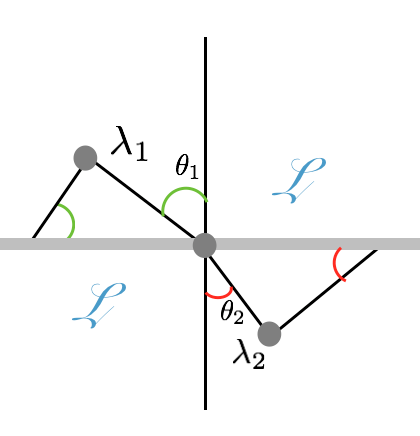
\includegraphics[width = \linewidth]{snell.png}
\caption{Illustration de la loi de Snell, les deux longueurs doivent être identiques}
\end{marginfigure}

Nous obtenons alors la \textbf{Loi de Snell}, valable pour des milieux \textit{isotropes}, transparents (non-absorbants) et linéaires (le tout à la fois!) :
\[ n_{1} \sin(\theta_{1}) = n_{2} \sin(\theta_{2})\]

Cette loi prédit les \textit{directions} des ondes réfléchies et transmises, mais ne dit rien quant à leur \textsl{amplitude} (ou leur énergie). 

\subsection{Equations de Fresnel}

Les \textbf{équations de Fresnel}, sur base des conditions aux interfaces pour les champs électriques et magnétiques, permettent de caractériser les amplitudes des ondes réfléchies et transmises. \\ 
Il est important de se souvenir de l'\textit{impédance caractéristique} qui quantifie le rapport des normes des champs électriques et magnétiques. Nous allons traiter uniquement du cas le plus courant, celui des ondes planes \textit{transverses}, afin de faciliter la compréhension de cette matière\footnote{Un raisonnement analogue peut-être entrepris concernant les ondes longitudinales.

Enormément de paramètres seraient inversés et les conditions de continuité seraient différentes.}.

Tout d'abord, la relation permettant de calculer (de \textit{manière générale} ici) un champ en fonction de l'autre\footnote{Par convention, la direction de $\vec{H}$ est ($\hat{k} \times \vec{E}$) et la direction de $\vec{E}$ est 
($ \vec{H} \times \hat{k}$) } : 

\[\vec{H}(\vec{r},t) = \frac{1}{Z}\vec{1_k} \times \vec{E}(\vec{r},t) \] %= \frac{n}{c\epsilon}\vec{H}(\vec{r},t) = \frac{c\mu}{n}\vec{H}(\vec{r},t)\]

Nous pouvons alors décomposer ce dernier en une composante \textit{parallèle} au plan d'incidence et une autre \textit{perpendiculaire} à ce dernier. La composante appartenant au plan d'incidence peut elle même être décomposée comme montré sur la figure \ref{decomp}, dans le plan $xz$.

Nous pouvons décomposer chaque onde selon trois composantes polarisées linéairement dans les directions $\hat{x}, \hat{y}, \hat{z}$ sur la figure. \\
Dès lors, nous allons pouvoir réappliquer les concepts vus avec la corde vibrante concernant l'amplitude de chacune de ces composantes. Il est avant tout important de spécifier les conventions prises pour la suite. Celles-ci sont précisées aux figures \ref{fig_convention1}, \ref{fig_convention2} et \ref{decomp}.
\begin{marginfigure}[-4cm]
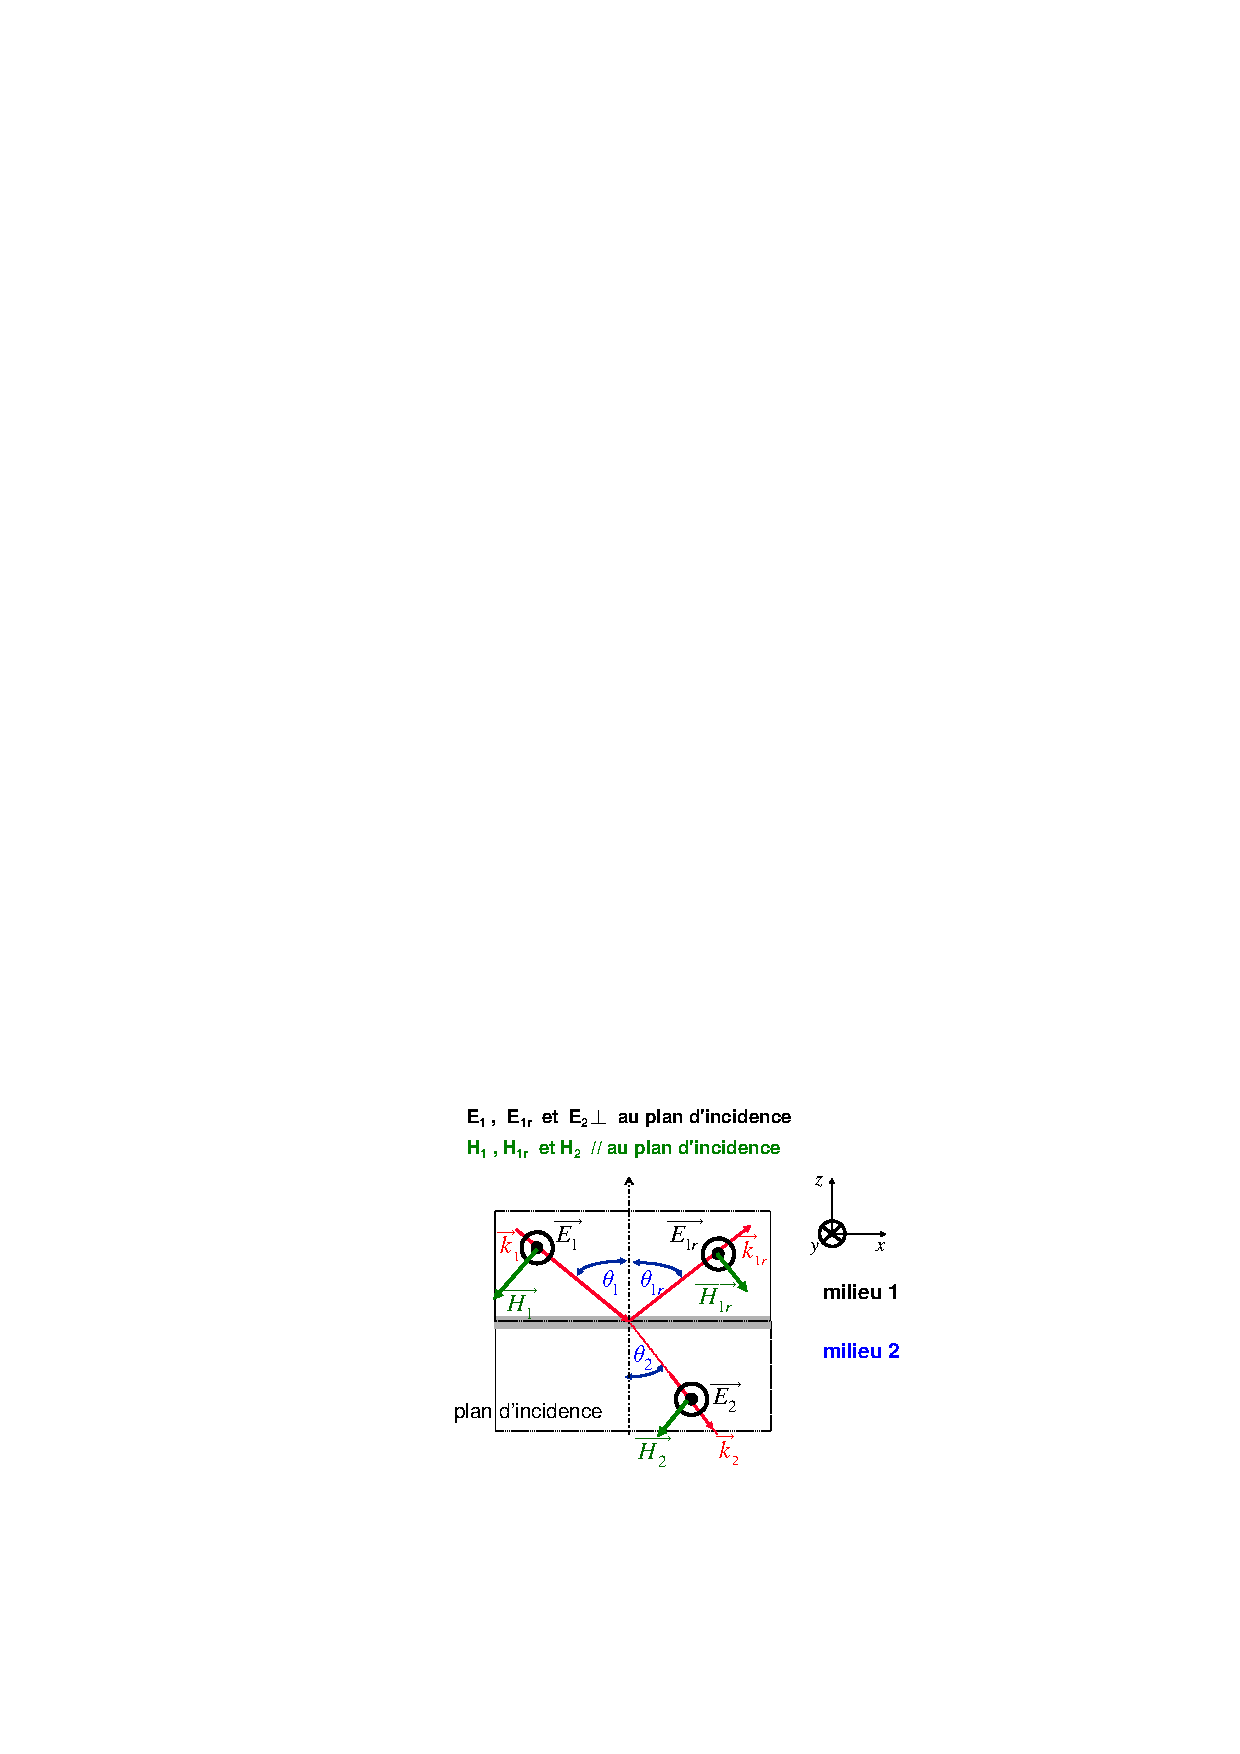
\includegraphics[width=\linewidth]{convention1}
\caption{Convention prise pour les champs électriques incidents parallèles à l'interface}
\label{fig_convention1}
\end{marginfigure}

 Commençons par écrire les ondes \textit{réfléchie} et \textit{transmise} en fonction de l'onde \textit{incidente}.\\
\textbf{Incidente:} $$ \vec{E}_{1i} (\vec{r},t) = (E^{\parallelsum}_{1i} \cos(\theta_{1})  \hat{x} + E_{1i}^{\perp} \hat{y} + E_{1i}^{\parallelsum} \sin(\theta_{1}) \hat{z} ) \sin(\vec{k}_{1i}\cdot \vec{r} - \omega t) $$  
\textbf{Réfléchie:}  $$ \vec{E}_{1r} (\vec{r},t) = (E^{\parallelsum}_{1r} \cos(\theta_{1})  \hat{x} + E_{1r}^{\perp} \hat{y} - E_{1r}^{\parallelsum} \sin(\theta_{1}) \hat{z} ) \sin(\vec{k}_{1r}\cdot \vec{r} - \omega t) $$
\textbf{Transmise:}$$ \vec{E}_{2t} (\vec{r},t) = (E^{\parallelsum}_{2t} \cos(\theta_{2})  \hat{x} + E_{2t}^{\perp} \hat{y} + E_{2t}^{\parallelsum} \sin(\theta_{2}) \hat{z} ) \sin(\vec{k}_{2t}\cdot \vec{r} - \omega t) $$ 
 
Notons que $\vec{k_{1r,z}} = - \vec{k_{1i,z}}$ et que $\vec{k_{2t}}$ prolonge l'angle de \textit{réfraction} en ayant, pour rappel, une norme de $\frac{\omega}{v_{2}}$.
Notons également que résoudre le problème pour le champ électrique nous permettra également de calculer le champ magnétique par la relation énoncée plus haut.
Toutefois, il nous faut également les expressions des champs $\vec{H}(\vec{r},t)$ afin de posséder assez d'équations.

\begin{marginfigure}
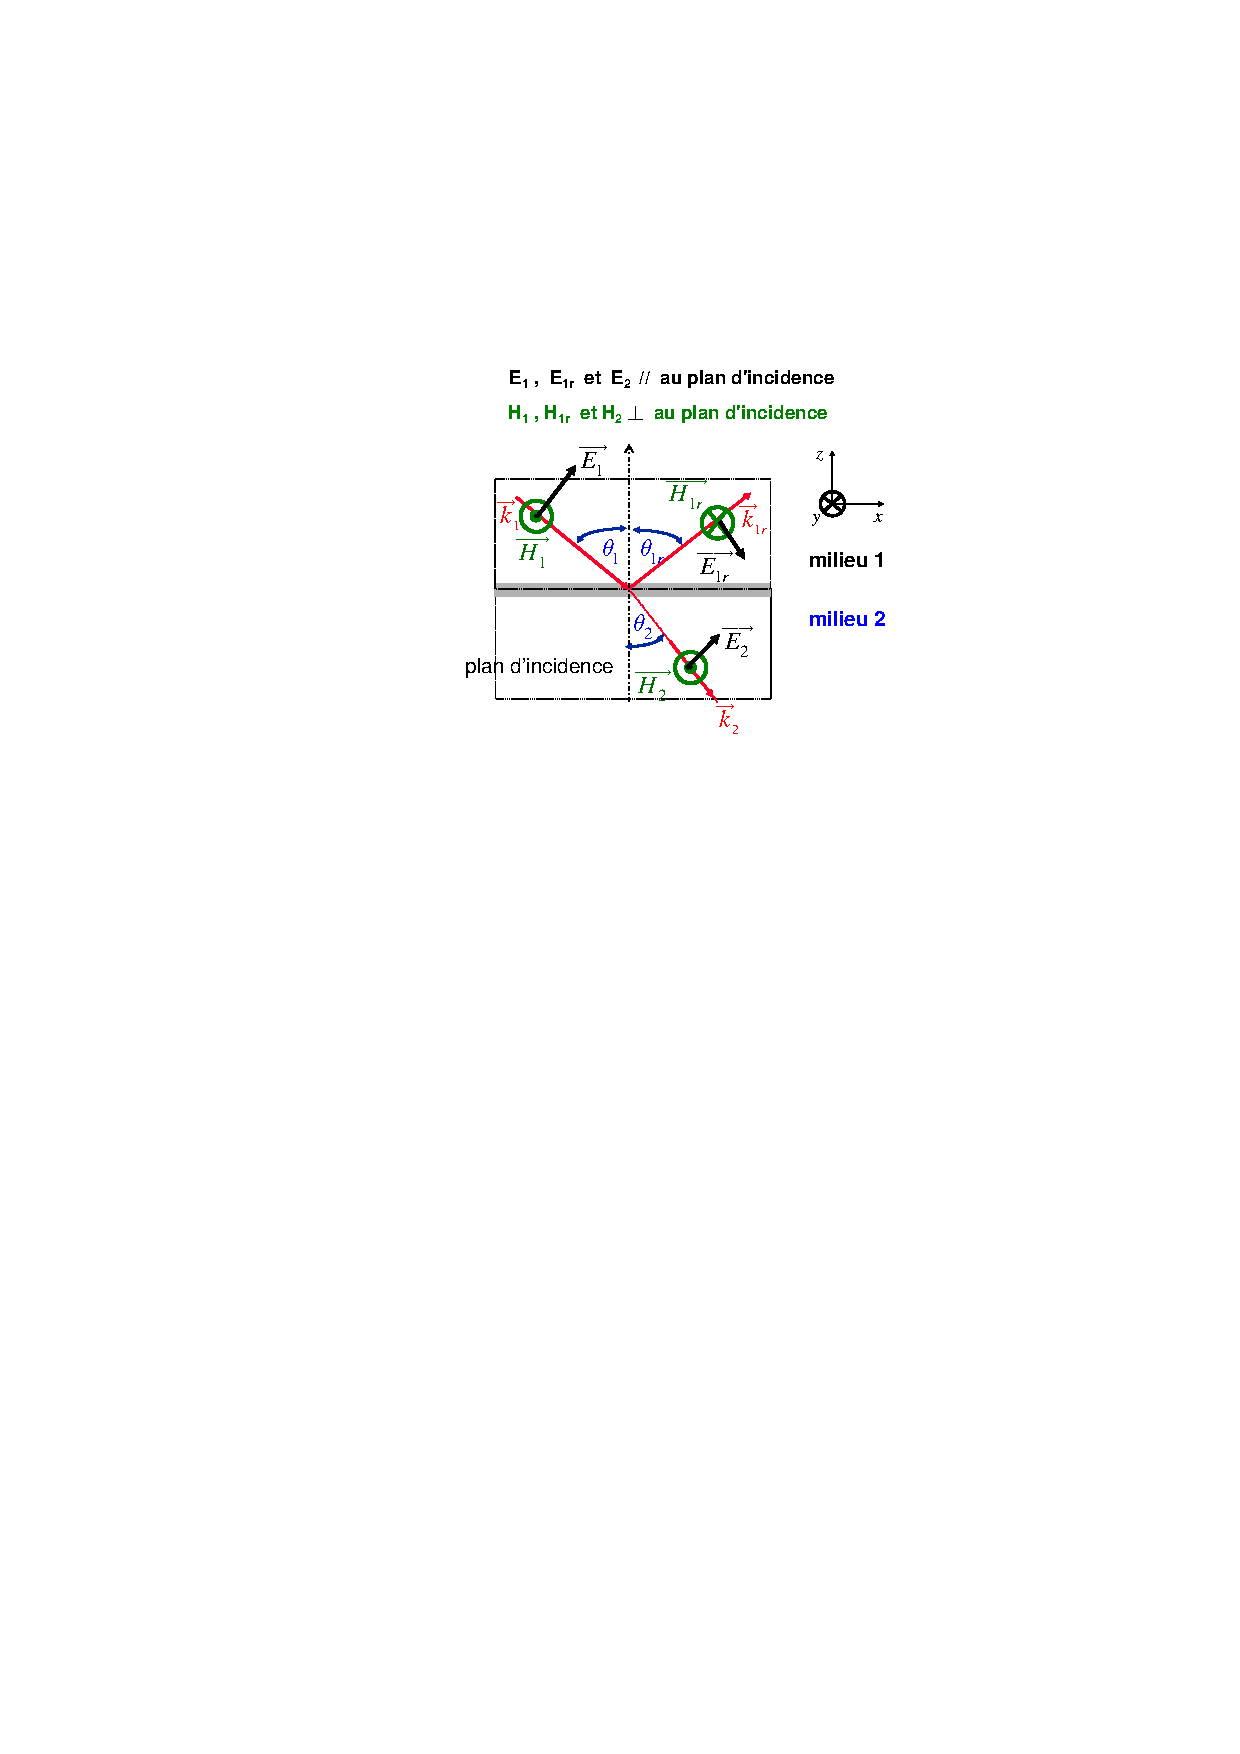
\includegraphics[width=\linewidth]{convention2}
\caption{Convention prise pour les champs H incidents parallèles à l'interface}
\label{fig_convention2}
\end{marginfigure}
\begin{marginfigure}
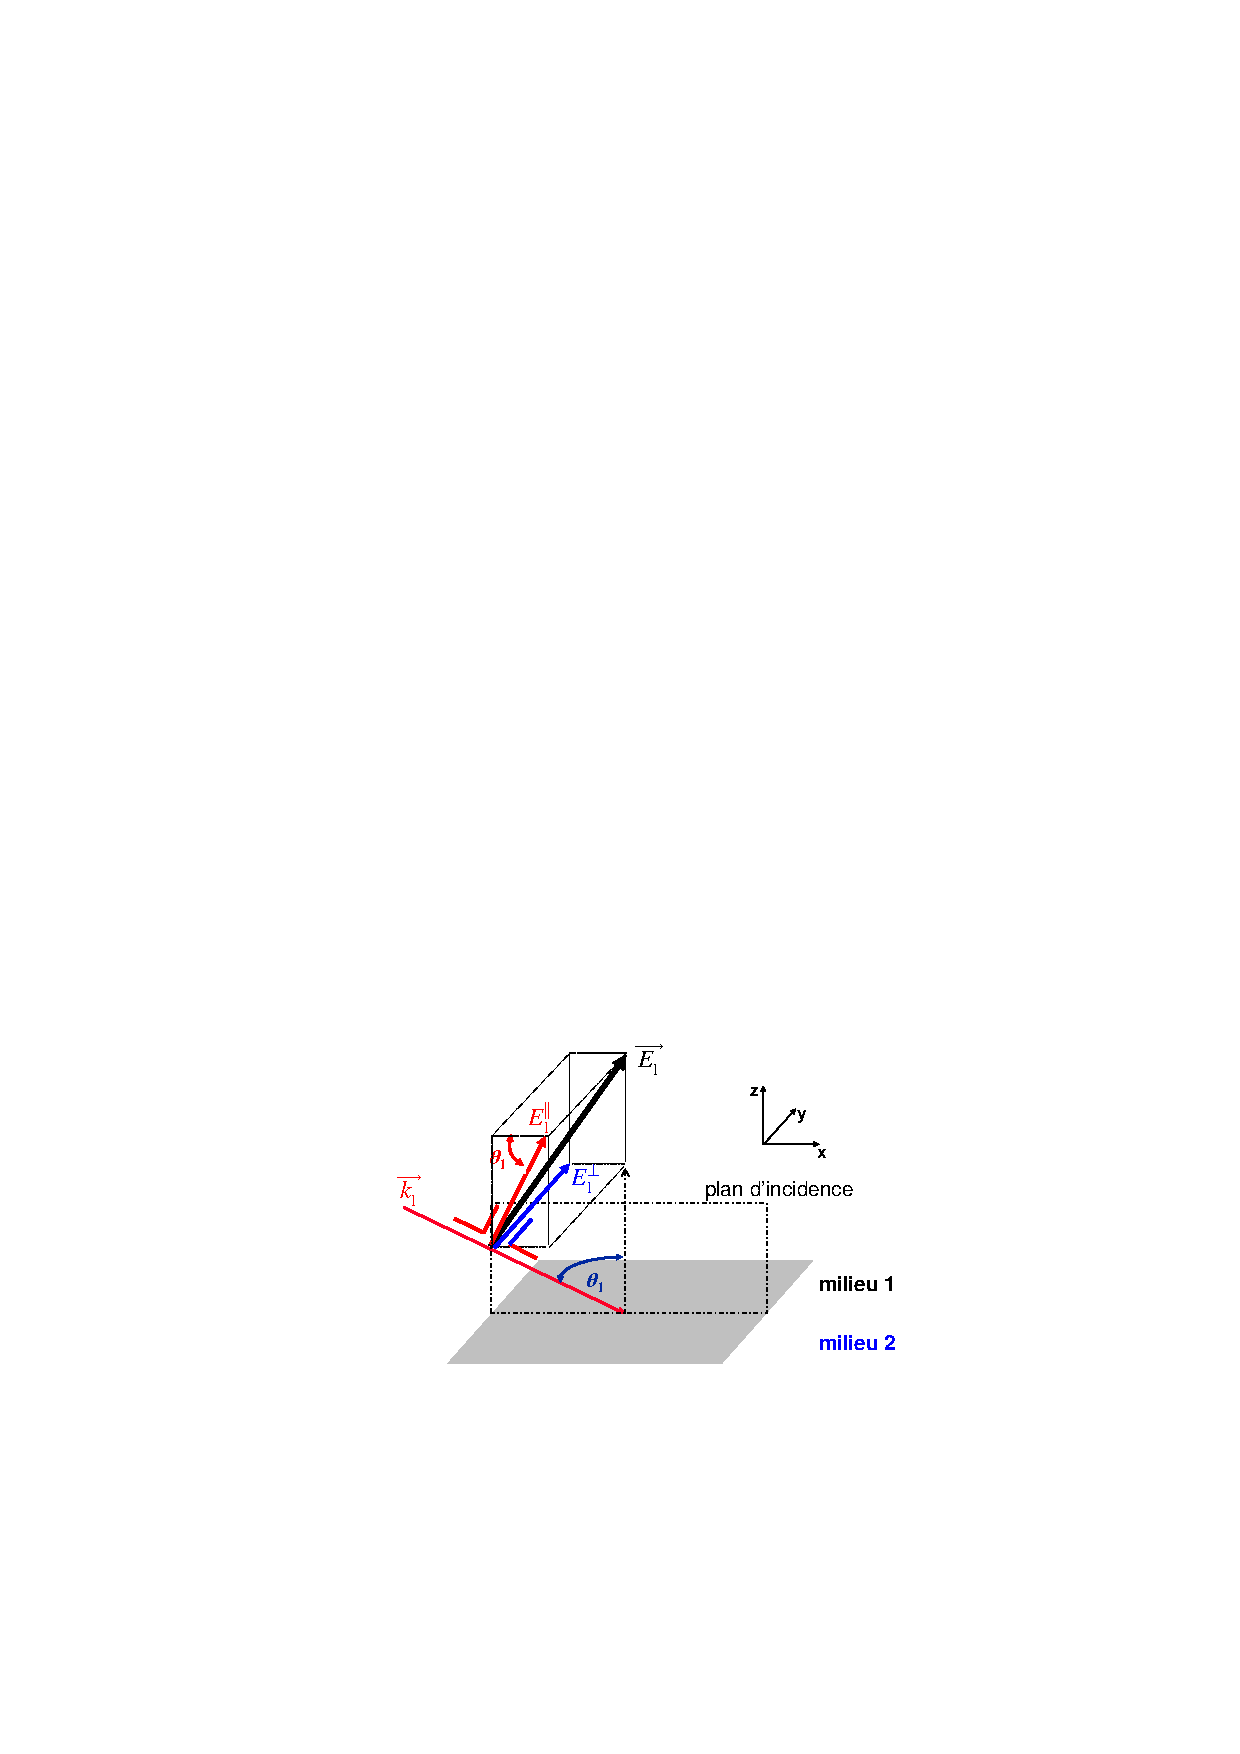
\includegraphics[width=\linewidth]{CM4_planincident}
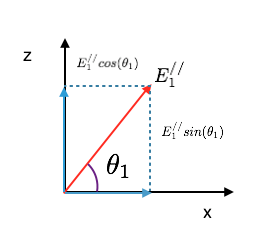
\includegraphics[width=\linewidth]{explicationsmall}
\caption{Décomposition du vecteur champ électrique par rapport au plan incident (haut) et projection du vecteur // au plan incident sur le plan xz (bas)}
\label{decomp}
\end{marginfigure}

Etant donné que $\hat{k_{1i}} = (\sin(\theta_{1}),0,-\cos(\theta_{1})) $, l'expression du champ magnétique incident se calcule et donne :
\begin{equation*}
\begin{split}
\vec{H}_{1i}(\vec{r},t)& = \frac{1}{Z_1} (\hat{k_{1i}} \times \vec{E}_{1i}(\vec{r},t))\\ &= \frac{1}{Z_1} \sin(\vec{k}_{1i}\cdot \vec{r} - \omega t)(E^{\perp}_{1i}\cos(\theta_{1}) \hat{x} - E^{\parallelsum}_{1i} \hat{y} + E^{\perp}_{1i}\sin(\theta_{1}) \hat{z} )
\end{split}
\end{equation*}
Les ondes incidente, réfléchie et transmise sont donc :\\ 
\textbf{Incidente} $$ \vec{H}_{1i} (\vec{r},t) = (E^{\perp}_{1i}\cos(\theta_{1}) \hat{x} - E^{\parallelsum}_{1i} \hat{y} + E^{\perp}_{1i}\sin(\theta_{1}) \hat{z} ) \frac{1}{Z_1} \sin(\vec{k}_{1i}\cdot \vec{r} - \omega t)$$

\textbf{Réfléchie} $$ \vec{H}_{1r} (\vec{r},t) = (-E^{\perp}_{1r} \cos(\theta_{1})  \hat{x} + E_{1r}^{\parallelsum} \hat{y} + E_{1r}^{\perp} \sin(\theta_{1}) \hat{z} ) \frac{1}{Z_1} \sin(\vec{k}_{1r}\cdot \vec{r} - \omega t) $$

\textbf{Transmise} $$ \vec{H}_{2t} (\vec{r},t) = (E^{\perp}_{2t} \cos(\theta_{2})  \hat{x} - E_{2t}^{\parallelsum} \hat{y} + E_{2t}^{\perp} \sin(\theta_{2}) \hat{z} ) \frac{1}{Z_2}\sin(\vec{k}_{2t}\cdot \vec{r} - \omega t) $$
 
Nous abordons alors réellement les équations de Fresnel.
%\footnote{Si vous désirez de plus amples informations sur ce qui a été dit et tout ce qui suivra, vous pouvez consulter le site suivant : \url{http://www.edu.upmc.fr/physique/phys325/Documents/Reflexion-Refraction.pdf}.}.
 La somme vectorielle des champs électriques en $\hat{x}$ 
du milieu 1 (à savoir ceux dans cette même direction pour l'onde incidente et réfléchie) doit être équivalente à celle du milieu 2 (à savoir l'onde transmise).%DONE\todo{CORRIGER LE SCHEMA : Ne respecte pas les conventions des slides (pages 16 et 17 CM4) le reste a été adapté. Mettre a la place du schema les fig 1 et 2 issues des slides, elles sont les plus adaptées}

%%% PROFESSEURS : Si nous plaçons un champ électrique à proximité de l'interface, jouera t'il un rôle dans la continuité de celui ci aux interfaces? Peut-on brouiller en quelque
%%% sorte ce qu'il se passe aux interfaces de quelque manière que cela soit? 

%\begin{center}
%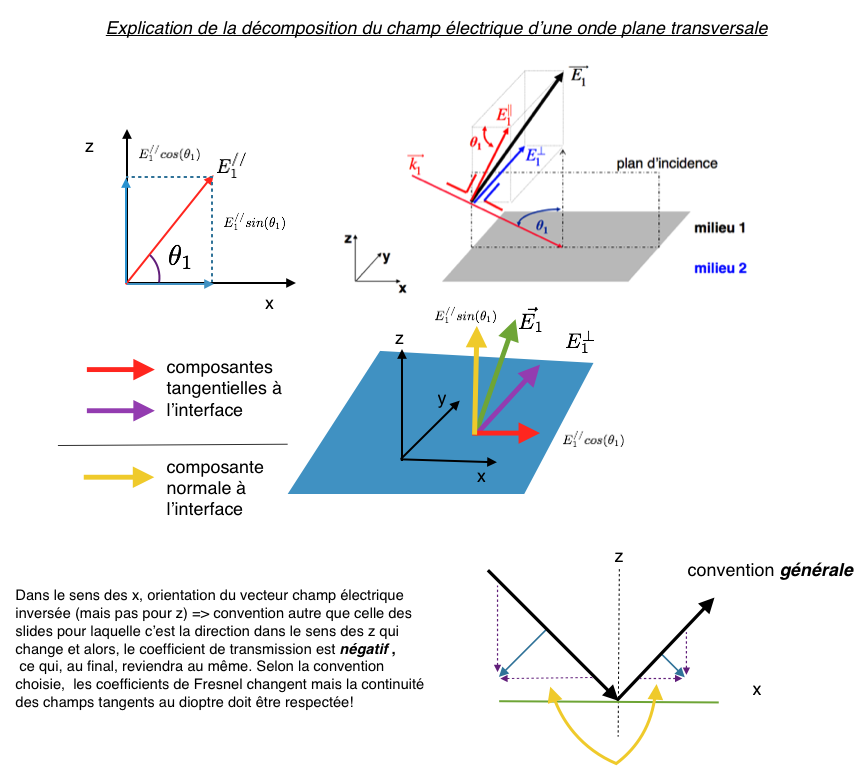
\includegraphics[height = 400pt,width = 450pt]{explicationbig.png}
%\end{center}


Nous écrivons sans peine en partant des composantes en $\hat{x}$ et des $\hat{y}$ les 4 conditions de continuité à l'interface du dioptre. Pour cela, il faut se rappeler le chapitre 1, dans lequel nous avons mentionné que les conditions limites aux interfaces imposaient que la partie tangentielle du champ E et du champ H soit conservée (en l'absence de charges et de courants à l'interface, ce qui est bien le cas ici). Nous devons donc imposer la continuité selon les axes $\hat{x}$ et $\hat{y}$. %\footnote{Claude dit NON: Nous adoptons la convention dénotée à la page précédente; celle du cours sera donnée juste après en titre de conclusion.} :  
\begin{equation*}
\begin{split}
\mbox{Continuité de $\vec{E}(\vec{r},t)$ selon $\hat{x}$ : }&\hspace{5pt} E^{\parallelsum}_{1i} \cos(\theta_{1}) +E^{\parallelsum}_{1r} \cos(\theta_{1}) = E^{\parallelsum}_{2t} \cos(\theta_{2})\\
\mbox{Continuité de $\vec{E}(\vec{r},t)$ selon $\hat{y}$ : }&\hspace{5pt} E_{1i}^{\perp} + E_{1r}^{\perp} = E_{2t}^{\perp}  \\
\mbox{Continuité de $\vec{H}(\vec{r},t)$ selon $\hat{x}$ : }&\hspace{5pt} Z_2E^{\perp}_{1i}\cos(\theta_{1}) - Z_2E^{\perp}_{1r} \cos(\theta_{1}) = Z_1E^{\perp}_{2t} \cos(\theta_{2})   \\
\mbox{Continuité de $\vec{H}(\vec{r},t)$ selon $\hat{y}$ : }&\hspace{5pt} -Z_2E^{\parallelsum}_{1i} + Z_2E_{1r}^{\parallelsum} = -Z_1E_{2t}^{\parallelsum}
\end{split}
\end{equation*}
  
où $E_{1i}^{\parallelsum}$, $E_{1i}^{\perp}$, $\theta_{1}$,$\theta_{2}$, $Z_1$ et $Z_2$ sont connus.

Nous pouvons établir un système matriciel étant donné le caractère \textit{linéaire} des équations.
%\begin{fullwidth}
%\begin{center}
	$$
	\begin{pmatrix}
	-\cos \theta_{1} & 0 & \cos \theta_{2}& 0\\
	0 & -1 & 0 & 1\\
	0 & Z_2\cos \theta_{1} & 0 & Z_1\cos \theta_{2}\\ 
	Z_2 & 0 & -Z_1 & 0
	\end{pmatrix}
	\cdot
	\begin{pmatrix}
	E_{1r}^{\parallelsum}\\
	E_{1r}^{\perp}\\
	E_{2t}^{\parallelsum} \\ 
	E_{2t}^{\perp}
	\end{pmatrix}
	=
	\begin{pmatrix}
	E_{1i}^{\parallelsum} \cos \theta_{1}\\
	E_{1i}^{\perp} \\
	Z_2E_{1i}^{\perp} \cos \theta_{1} \\
	Z_2E_{1i}^{\parallelsum}
	\end{pmatrix}
	$$
%\end{center}
%\end{fullwidth}
%\vspace{10pt}
Nous pouvons résoudre ce système d'équations et obtenir les 4 coefficients de Fresnel suivants:
\[r_{\parallelsum} \overset{\Delta}= \frac{E_{1r}^{\parallelsum}}{E_{1i}^{\parallelsum}} = \frac{Z_{2}\cos \theta_{2} - Z_{1} \cos \theta_{1} }{Z_{2} \cos \theta_{2} + Z_{1} \cos \theta_{1} } \]
\[r_{\perp} \overset{\Delta}= \frac{E_{1r}^{\perp}}{E_{1i}^{\perp}} = \frac{Z_{2}\cos \theta_{1} - Z_{1} \cos \theta_{2} }{Z_{2} \cos \theta_{1} + Z_{1} \cos \theta_{2}}\]
\[t_{\parallelsum} \overset{\Delta}= \frac{E_{2t}^{\parallelsum}}{E_{1i}^{\parallelsum}} = \frac{2 Z_{2} \cos \theta_{1} }{Z_{2} \cos \theta_{2} + Z_{1} \cos \theta_{1}} \]
\[t_{\perp} \overset{\Delta}= \frac{E_{2t}^{\perp}}{E_{1i}^{\perp}} = \frac{2 Z_{2} \cos \theta_{1} }{Z_{2} \cos \theta_{1} + Z_{1} \cos \theta_{2}}\]
Ces coefficients sont valables dans les milieux avec une permittivité électrique et une perméabilité magnétique constantes. La forme des équations de Fresnel ici présentes n'est pas unique. En effet, il existe des équations de Fresnel sous une forme plus restrictive. Cette forme n'utilise pas les impédances des deux milieux mais leur indice de réfraction. Elle est utilisée couramment chez des opticiens pour cette raison. L'inconvénient est que ladite forme n'est valable que pour des milieux dont la perméabilité magnétique est celle du vide (autrement dit, pour des matériaux non-magnétiques): $Z_i = 1/n_i$. Pour les opticiens, il ne s'agit pas d'un problème car la plupart des matériaux utilisés en optique sont non-magnétiques. Dans le cadre de ce cours, nous utiliserons toujours de préférence les formules énoncées plus haut. Néanmoins, voici les équations de Fresnel avec les indices de réfraction: 
\sidenote[][-5cm]{Afin de visualiser la réflexion et la réfraction au mieux,  il existe deux animations \textit{Matlab} très bien réalisées disponibles sur le site Moodle du cours.}% En prime\footnote{Disponible dans le fichier .zip}, un autre programme \textit{Matlab} vous permettant  de calculer rapidement les coefficients de \textit{Fresnel} suivant la convention du cours. Il est conseillé d'analyser la notice d'utilisation. \textbf{Notez} que si vous désirez afficher les graphes de l'évolution des coefficients de \textit{Fresnel} par rapport à l'angle incident; il vous faut simplement appeler la fonction avec le rapport $\frac{n_{1}}{n_{2}}$ souhaité entre les deux milieux. Enfin, ce programme est rapidement fait et n'est certainement pas optimisé ni défensif; il a pour but d'être le substitut à une calculette un peu longue à manier pour des calculs de \textit{coefficients de Fresnel}.}:  

\[r_{\parallelsum} \overset{\Delta}= \frac{E_{1r}^{\parallelsum}}{E_{1i}^{\parallelsum}} = \frac{n_{1}\cos \theta_{2} - n_{2} \cos \theta_{1} }{n_{2} \cos \theta_{1} + n_{1} \cos \theta_{2} } = \frac{\tan(\theta_{2}-\theta_{1})}{\tan(\theta_{1}+\theta_{2})}\]
\[r_{\perp} \overset{\Delta}= \frac{E_{1r}^{\perp}}{E_{1i}^{\perp}} = \frac{n_{1}\cos \theta_{1} - n_{2} \cos \theta_{2} }{n_{2} \cos \theta_{2} + n_{1} \cos \theta_{1}} = -\frac{\sin(\theta_{1} - \theta_{2})}{\sin(\theta_{1} + \theta_{2})} \]
\[t_{\parallelsum} \overset{\Delta}= \frac{E_{2t}^{\parallelsum}}{E_{1i}^{\parallelsum}} = \frac{2 n_{1} \cos \theta_{1} }{n_{2} \cos \theta_{1} + n_{1} \cos \theta_{2}} \]
\[t_{\perp} \overset{\Delta}= \frac{E_{2t}^{\perp}}{E_{1i}^{\perp}} = \frac{2 n_{1} \cos \theta_{1} }{n_{2} \cos \theta_{2} + n_{1} \cos \theta_{1}}\]

%\subsection{Convention du cours: NON: il faut directeemnt utiliser la bonne convention, dit Claude}

%En ce qui concerne la convention du cours, il est seulement nécessaire de modifier le signe du coefficient $r_{//}$ ainsi que le signe des composantes en $\hat{x}$ et en $\hat{z}$ de tous les champs réfléchis et transmis dont nous parlions ci-dessus. 
Les deux formes des coefficients de Fresnel sont évidemment équivalentes si $\mu_1 = \mu_2 = \mu_0$. Il est aussi possible de rencontrer dans la littérature d'autres formes pour les équations de Fresnel, résultant d'une convention différente prise pour le sens dit positif des champs. 
%\todo{Analyser les graphes p21 et suivants dans CM4, + dire ce que veut dire le signe du coeff de Fresnel, car les champs etant alternatifs, le signe du coeff de Fresnel indique si les champs sont en phase tels que dessinés ou pas, et rien d'autre; si on change le sens des conventions, le signe du coeff change; mais ne pas oublier que les champs changent de sens toutes les demi-periodes ... }
\section{Conséquences des équations de Fresnel}
Supposons une interface entre deux milieux non-magnétiques (pour simplifier l'analyse), par exemple, une interface air-lucite (la lucite est le nom correct du plexiglas, qui est à la base une marque de produit).

Lorsqu'une onde EM passe de l'air vers la lucite, à incidence normale ($\theta_1=0^\circ$ sur la figure \ref{fig_ref2}), nous remarquons que les coefficients de réfraction sont négatifs. \textit{La réflexion change donc le sens du champ électrique} en lui appliquant un déphasage de $180^\circ$.\sidenote{Attention, il ne s'agit pas d'une histoire de conventions, le déphasage est bien réel. Pour s'en convaincre, il suffit de regarder les figures \ref{fig_convention1} et \ref{fig_convention2} en imaginant $\theta_1=0^\circ$. Nous pouvons remarquer que dans ce cas les vecteurs se confondent.} Avec une analyse similaire, on peut déterminer que la transmission ne change pas le sens du champ électrique.

Toujours dans le même cas (air $\rightarrow$ lucite), nous observons qu'à incidence rasante ($\theta_1$ proche de $90^\circ$), le coefficient de réflexion tend vers 1 et le coefficient de transmission vers zéro. \textit{A incidence rasante, la réflexion est totale.}\\

Dans le cas inverse, visible à la figure \ref{fig_ref3}, où $n_1>n_2$ (lucite $\rightarrow$ air), nous pouvons observer que tant le champ électrique transmis que réfléchi est du même sens que le champ électrique incident. Une remarque importante s'impose quant à la définition du sens des champs. Ces champs sont des ondes sinusoïdales, dont l'orientation change toutes les demi-périodes. Par sens, on entend bien le sens pris au même moment, à l'interface. Autrement dit, si un coefficient de Fresnel est positif pour les sens définis aux figures \ref{fig_convention1} et \ref{fig_convention2}, cela signifie qu'à un moment fixé, au point de réflexion, les champs ont le sens tel qu'indiqué sur la figure. Une demi-période plus tard, les champs seront tous (en même temps) dans le sens opposé. 

\section{Angles particuliers}
\begin{marginfigure}[-4cm]
	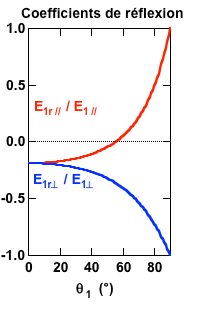
\includegraphics[width=\linewidth]{ref2}
	\caption{Coefficients de réflexion parallèle et perpendiculaire lorsque $n_1<n_2$ (air $\rightarrow$ lucite)}
	\label{fig_ref2}
\end{marginfigure} 
\begin{marginfigure}[0cm]
	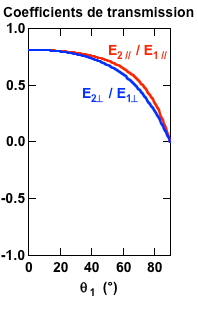
\includegraphics[width=\linewidth]{trans2}
	\caption{Coefficients de transmission parallèle et perpendiculaire lorsque $n_1<n_2$ (air $\rightarrow$ lucite)}
	\label{fig_trans2}
\end{marginfigure} 

\subsection{Angle de \textit{Brewster} et transmission totale}

Nous pouvons remarquer que le coefficient $r_{\parallelsum}$ peut s'annuler dans le cas particulier où $Z_2\cos\theta_{2} = Z_1\cos\theta_{1}$, autrement dit lorsque 
\[\sin^2\theta_1 = \frac{\mu_2\epsilon_1/\mu_1\epsilon_2 - 1}{(\epsilon_1/\epsilon_2)^2-1}\]

Pour des milieux non-magnétiques ($\mu_1 = \mu_2 = \mu_0$), cela revient à 
\[\sin\theta_1 = (\epsilon_1/\epsilon_2+1)^{-1/2}\]

Cet angle $\theta_1$ est appelé \textit{angle de Brewster} et se note $\theta_{B}$.

Nous pouvons également retrouver cet angle (pour des milieux non-magnétiques) à partir de l'expression optique du coefficient $r_{\parallelsum}$ : 
\[\frac{n_{2}\cos \theta_{1} - n_{1} \cos \theta_{2} }{n_{2} \cos \theta_{1} + n_{1} \cos \theta_{2} } = 0 \Leftrightarrow n_{2} \cos \theta_{1} = n_{1} \cos \theta_{2} \Rightarrow \cos^{2} \theta_{2} = \left(\frac{n_{2} \cos \theta_{1}}{n_{1}}\right)^{2}\]
En utilisant la loi de \textit{Snell-Descartes} : 
\[n_{1} \sin \theta_{1} = n_{2} \sin \theta_{2} \Rightarrow \sin^{2} \theta_{2} = \left(\frac{n_{1} \sin \theta_{1}}{n_{2}}\right)^{2} \] 
En se souvenant de l'identité trigonométrique de base $ \cos^{2} \alpha + \sin^{2} \alpha = 1$ : 
\[\sin^{2} \theta_{1} + \cos^{2} \theta_{1} = \left(\frac{n_{1} \sin \theta_{1}}{n_{2}}\right)^{2} +  \left(\frac{n_{2} \cos \theta_{1}}{n_{1}}\right)^{2}\]
\[\sin^{2} \theta_{1} \left(\frac{n_{2}^{2} - n_{1}^{2}}{n_{2}^{2}}\right) = \cos^{2} \theta_{1} \left(\frac{n_{2}^{2} - n_{1}^{2}}{n_{1}^{2}}\right)\]
Enfin, nous pouvons écrire : 
\[\tan^{2} \theta_{1} = \frac{n_{2}^{2}}{n_{1}^{2}} \Rightarrow \theta_{1} \overset{\Delta}= \theta_{B} = \arctan\left(\frac{n_{2}}{n_{1}}\right)\]

De la même manière, on peut calculer l'angle pour lequel $r_{\perp}$ s'annule. On montre facilement que dans ce cas, un angle de Brewster n'existe que si les milieux sont magnétiques. Pour des milieux non-magnétiques, il n'y a jamais de transmission totale lorsque l'onde est polarisée perpendiculairement au plan d'incidence. 

Ces principes sont à la base du fonctionnement des polariseurs, c'est-a-dire des dispositifs produisant de la lumière polarisée. Si un rayonnement électromagnétique comportant une égale quantité des deux polarisations rencontre une interface entre deux milieux non-magnétiques sous un angle égal à l'angle de Brewster, la transmission sera totale pour la fraction de l'onde polarisée parallèlement au plan d'incidence, et partielle pour l'autre. On a donc polarisé l'onde transmise, en modifiant sa polarisation. De manière tout à fait générale, \textbf{l'état de polarisation} d'une onde change suite à une réfraction ou une réflexion en ce sens où l'amplitude des différentes composantes polarisées a été modifiée par les coefficients de \textit{Fresnel}. 

%\begin{center}
%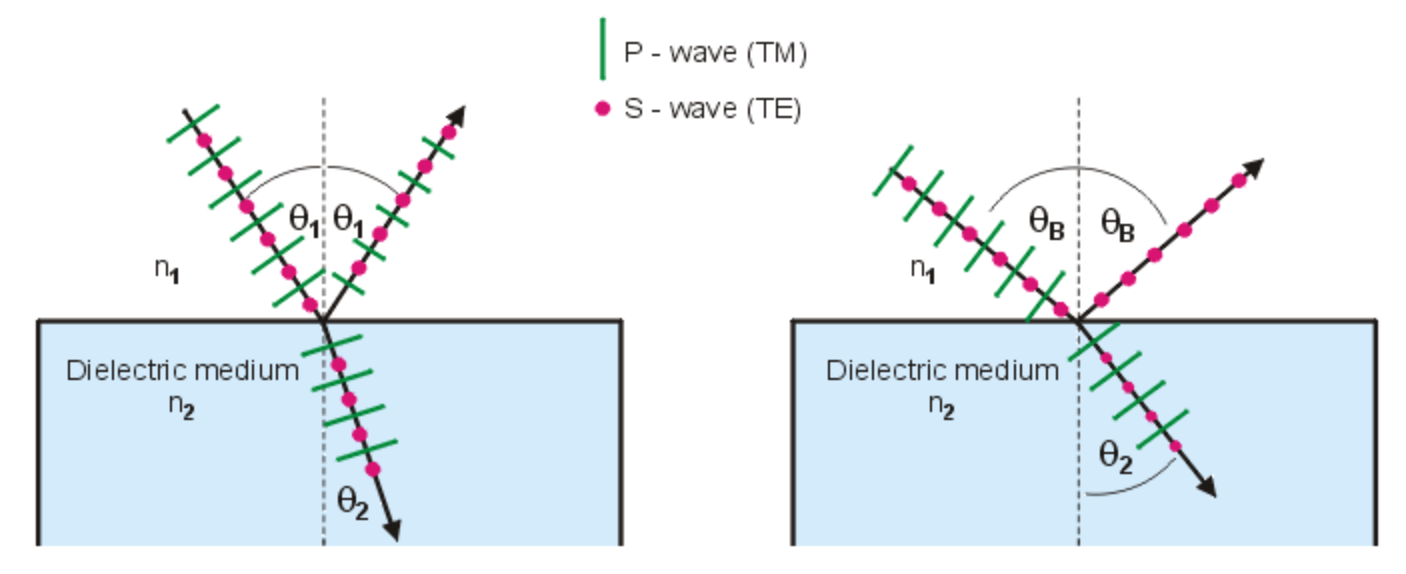
\includegraphics[height = 175pt, width = 300pt]{brewster.png}
%\end{center}

\begin{marginfigure}[-19cm]
	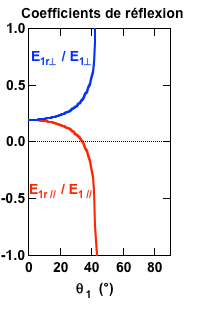
\includegraphics[width=\linewidth]{ref1}
	\caption{Coefficients de réflexion parallèle et perpendiculaire lorsque $n_1>n_2$ (lucite $\rightarrow$ air)}
	\label{fig_ref3}
\end{marginfigure} 

\subsection{Angle critique et réflexion totale}
\begin{marginfigure}[-5cm]
	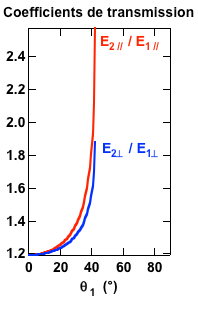
\includegraphics[width=\linewidth]{trans1}
	\caption{Coefficients de transmission parallèle et perpendiculaire lorsque $n_1>n_2$ (lucite $\rightarrow$ air)}
\end{marginfigure} 
Lorsque le milieu où s'opère la \textit{transmission} admet un indice de réfraction $n_{2}<n_{1}$, il existe un \textit{angle critique} d'incidence à partir duquel la réflexion est \textit{\textbf{totale}}, c'est-à-dire un angle au-delà duquel l'angle $\theta_2$ devient complexe et n'existe donc pas (pour un angle d'incidence égal à cet angle critique, $r_{\parallelsum}$ et $r_{\perp}$ sont égaux à  -1 et 1 respectivement; au delà de cet angle critique, les coefficients de Fresnel ne sont évidemment pas définis). 

Il faut noter que ce phénomène intervient quelle que soit la polarisation de l'onde incidente, pour des milieux magnétiques ou non, mais n'est possible qu'en passant d'un milieu plus réfringent à un milieu moins réfringent ($n_{2} < n_1$), par exemple, de la lucite (ou de l'eau, ...) vers l'air.

Par l'approche des coefficients de \textit{Fresnel}, nous remarquons tout de suite que \textit{l'angle critique} est l'angle d'incidence $\theta_{1} = \theta_{c}$ pour lequel l'angle de réfraction vaut $\frac{\pi}{2}$, ce qui nous donne: 
\[\sin \theta_{c} = \frac{n_{2}}{n_{1}} \Rightarrow \theta_{c} = \arcsin \left(\frac{n_{2}}{n_{1}}\right)\]
\begin{marginfigure}[-3cm]
	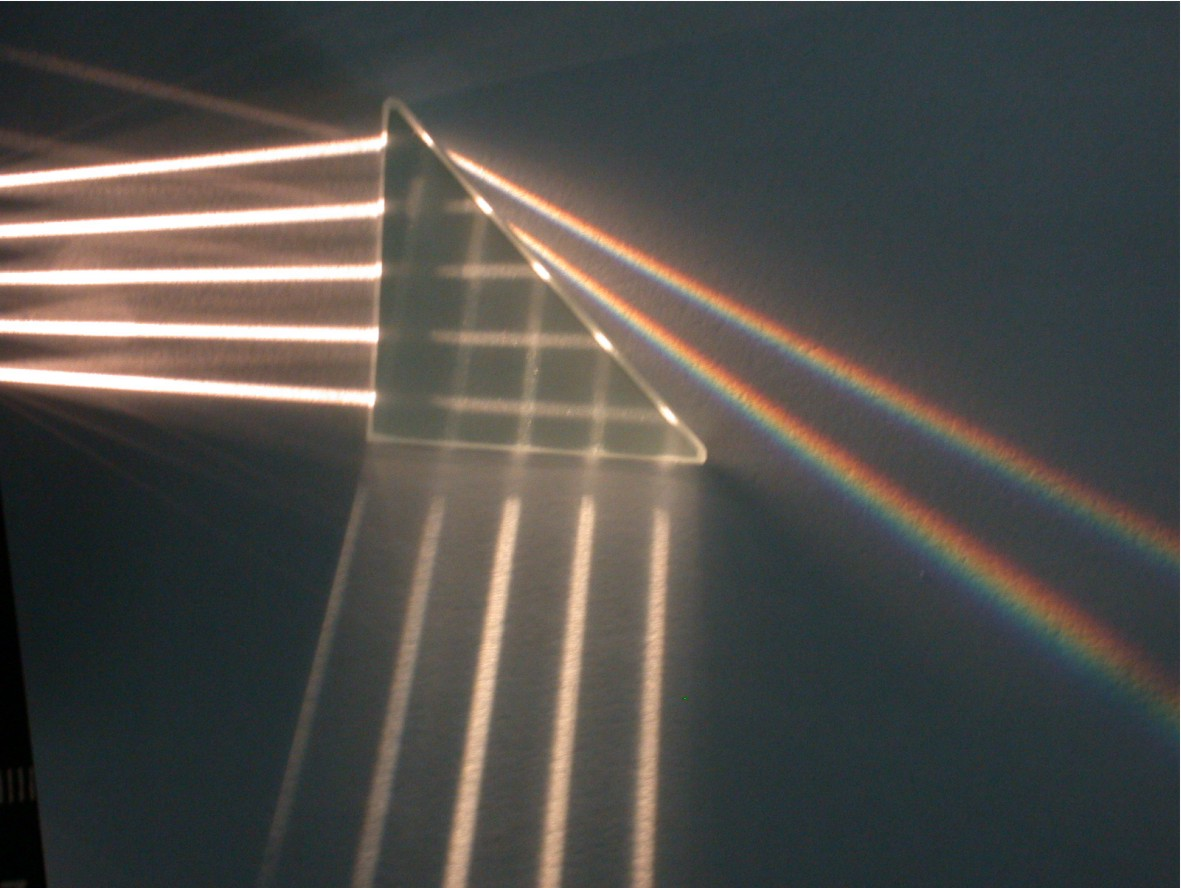
\includegraphics[width=\linewidth]{reflexion_tot}
	\caption{Illustration de la réflexion totale, les deux premières raies incidentes en partant du haut sont en dessous de l'angle critique, une partie de l'onde est donc transmise. A partir de la 3ème raie, plus aucune onde n'est transmise}
\end{marginfigure}
%\todo{De manière générale : Découper les schémas et les stacker verticalement pour utiliser l'espace sur la droite (marginfigure); refaire le schéma avec les conventions du cours ; importer le schéma des conventions slide p16; parler histoire?}
